\section{Introduction}

\lettrine[nindent=0em,lines=3]{S}{cripting} languages is an increasingly popular and important
category of programming languages. Programs written in scripting languages are often written for
a special run-time environment that can be automated through scripts--shells and Web browsers
are perhaps the two best known examples--or for a specialized domain, such as text processing.
JavaScript and Lua are examples of the former. JavaScript is used to extend the functionality
of Web pages displayed in a Web browser, while Lua is an extension language that is used in many 
commercial and free applications and is widely used in scripting video game engines. Lua is
often chosen for this task because it is designed to be very fast and easy to embed.
General-purpose scripting languages also exist and perhaps the most well-known one is Python.
Python is a widely-used, general-purpose high-level programming language that emphasizes code
readability whose syntax allows programmers to express concepts in fewer lines of code than would be 
possible in a language like C, enabling them to develop applications quicker. 
Scripting languages typically have a low barrier to entry and are easier for programers to 
get started with and provide a number of features that make them an important tool for increasing 
programmer productivity, and distinguish them from programming languages such as C, C++ and Java. 
For example, scripting languages are generally very high-level languages that provide a high level of 
abstraction. They are usually dynamically typed and provide automatic memory management. Many
scripting languages can load and execute code dynamically in the context of the running program
by passing a string consisting of program statements to an \texttt{exec()} function or something
similar.

In this report, we study and compare three different scripting languages, Python,
JavaScript, and Lua, and compare the similarities and differences of the features that
they offer. Our comparison of these three languages
is based on the implementation of a simple letter rearrangement game
called Letter Lizard. In the game, the player is presented with a set of letters and 
their goal is to form as many dictionary words as possible from the set of letters
before the timer runs out. In order to make the game
more engaging and enjoyable, we implemented a number of features that enable the user to customize
their gameplay experience by providing options to set the number of rounds, the time per round, 
and the level of difficulty for each
game.
%Although wanted to create a game that is fun and enjoyable, our primary objective was to
%compare and contrast the features of each programming language. 
We adhered to the same
design for each implementation while also using the idiomatic features of each language as much as 
possible. The game proceeds as follows:

\begin{itemize}
    \item On beginning the game, a welcome screen or a ``Splash Screen'' is displayed
    to the user. The user must hit the spacebar to proceed to the Main Menu screen.
    \item The Main Menu screen allows the user to configure game options, such as the
    number of rounds, time per round and level of difficulty. After setting these options, the
    user clicks \textbf{Start} to begin a new game and is taken to the main Game screen.
    \item The Game screen displays the set of letters to the user and allows them to type
    words that can be formed from the letters. It also shows the round number, the amount of
    time remaining, the user's score, and placeholders for all of the dictionary words that
    can be formed from the set of letters. After typing a word, the user hits
    enter and the game engine checks to see that the word is a valid dictionary word, and, if so,
    reveals the word in the list of placeholders. The Game screen also has options to shuffle
    the set of letters, generate a hint for a word yet to be found, and return to the main menu.
\end{itemize}

\begin{figure}
    \centering
    \begin{subfigure}{0.49\textwidth}
        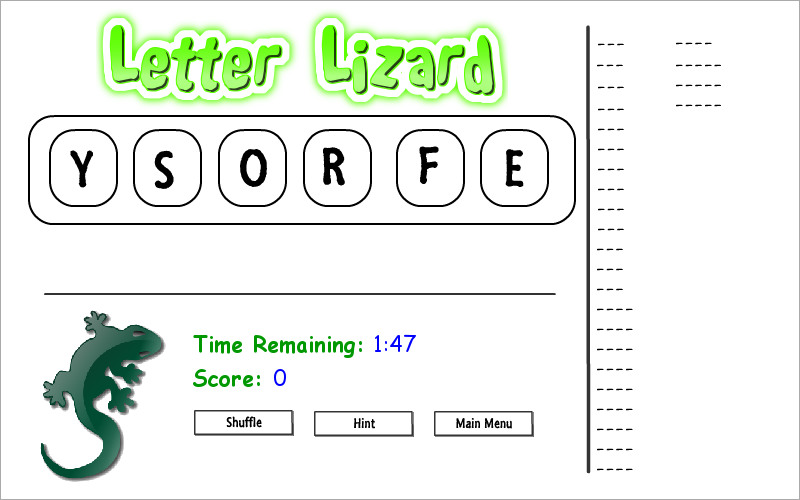
\includegraphics[width=\textwidth]{../mockups/Game_Screen.jpg}
        \caption{Main game screen mockup}
        \label{mainscreenmockup}
    \end{subfigure}
    \begin{subfigure}{0.49\textwidth}
        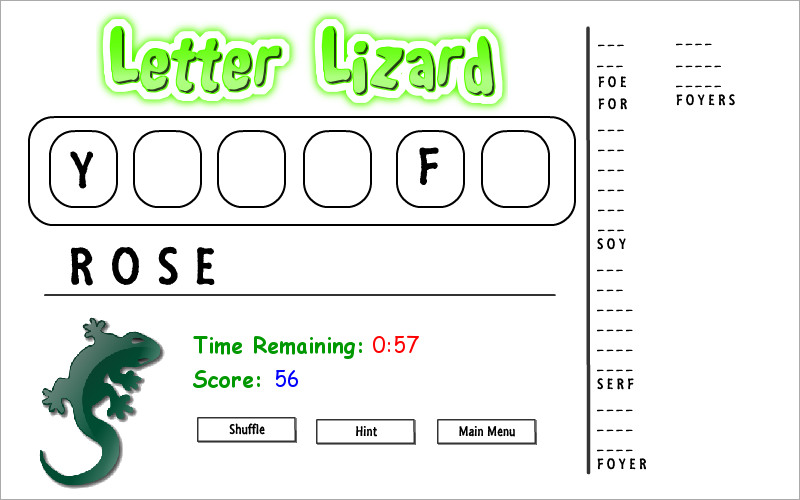
\includegraphics[width=\textwidth]{../mockups/Gameplay.jpg}
        \caption{Gameplay mockup}
        \label{gameplaymockup}
    \end{subfigure}
    \caption[Two mockups from our design document demonstrating the proposed Letter Lizard game]
    {Two mockups from our design document demonstrating the proposed Letter Lizard game
    showing (a) the main game screen and (b) the gameplay.}
    \label{mockups}
\end{figure}

All three implementations of Letter Lizard provide graphical user interfaces
that are modelled after the mockups presented in our design document. The mockups showing the
main game screen and gameplay are shown in Figure~\ref{mockups}. Additionally, the internal 
data structures and algorithms representing the game state and gameplay are similar 
in all three implementations.

The set of letters and collection of dictionary words can can be formed from the set of letters
is generated by a Python script called the \emph{game generator} that can be run as a standalone,
command line program or be imported as a module. The game generator works by loading a set
of dictionaries, generating a set of scrambled letters, and then finding dictionary words that can
be formed by the set of scrambled letters. When run as a stand alone program, the default output of the
tool is plain text where each line consists of the set of scrambled letters followed by all of the 
dictionary words that can be formed from those letters. Alternatively, the game generator can be provided
with command line parameters that cause it to output the list of letters and words as JavaScript or Lua 
source code that initializes an object or table with the letters and words.
The game generator accepts parameters that configure the
number of scrambled letters in each game, the number of games to generate, and the difficulty
of each game. The dictionary that we used (Spell Checking Oriented Word Lists by Kevin
Atkinson) is partitioned into words that are more frequently used and less frequently used in
common English. When choosing a harder difficulty, the list of words for the user to find will
contain more words that are used less frequently.
When generating the set of scrambled letters, the game generator picks each letter of the alphabet with a
probability corresponding to the frequency that it appears in the dictionary (which we
precomputed ahead of time). In order to find the dictionary words that can be formed, the game generator
iterates through the dictionary and checks to see if each dictionary word can be formed from the set of 
scrambled letters, and if so, it adds it to the list of words for the set of scrambled letters.

The next three sections introduce each language and discuss the Letter Lizard implementation in
that language. Section~\ref{comparison} compares the different features offered by each language using
examples from our three implementations. Section~\ref{conclusion} concludes by discussing which
language features made certain aspects of the game easier to implement and summarizes the features
that we found most useful.